\documentclass{beamer}
\usetheme{Warsaw}
\setbeamertemplate{footline}[frame number]

\usepackage[utf8]{inputenc}
\usepackage{fancybox}
\usepackage{multimedia} 
\usepackage{subfig}
\usepackage{amsmath}
\usepackage{hyperref}
\usepackage[all]{xy}
\begin{document}


\title[Angewandte Mathematik] % (optional, only for long titles)
{Angewandte Mathematik
\\

\includegraphics[scale=0.15]{images/cover}
}
\subtitle{}
\author[Dr. Johannes Riesterer] % (optional, for multiple authors)
{Dr.  rer. nat. Johannes Riesterer}

\date[KPT 2004] % (optional)
{}

\subject{Angewandte Mathematik}

\frame{\titlepage}


\begin{frame}
\framesubtitle{Algorithmus}
    \begin{block}{Algorithmus}
\begin{figure}[H]
      \centering
    
\includegraphics[width=0.7\textwidth]{images/algo}
      \caption{Quelle: Wikipedia}
\end{figure}
\end{block}

 \end{frame}




\begin{frame}
    \frametitle{Angewandte Mathematik}
\framesubtitle{}
    \begin{block}{Algorithmus Informell}
Ein Algorithmus ist eine eindeutige, endliche Handlungsvorschrift zur Lösung eines Problems oder einer Klasse von Problemen. Algorithmen bestehen aus endlich vielen, wohldefinierten Einzelschritten.
\end{block}
    \begin{block}{Algorithmus Formal}
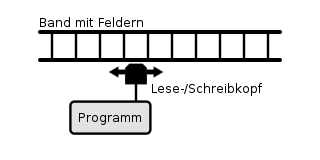
\includegraphics[scale=0.8]{images/Turingmaschine}
\end{block}
 \end{frame}

\begin{frame}
\framesubtitle{Algorithmus}
    \begin{block}{Algorithmus}
\begin{figure}[H]
      \centering
    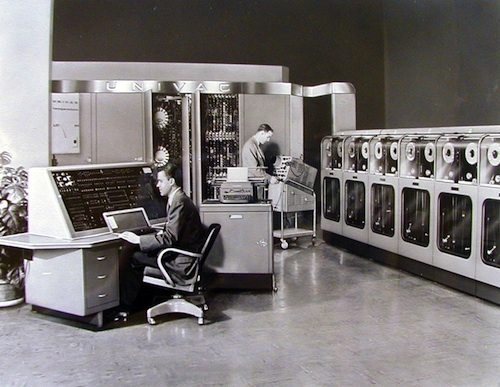
\includegraphics[width=0.7\textwidth]{images/computer}
      \caption{Quelle: Wikipedia}
\end{figure}
\end{block}

 \end{frame}






\begin{frame}
    \frametitle{Angewandte Mathematik}
\framesubtitle{Fehleranalyse}
    \begin{block}{Gleitkommazahl}
Eine Gleitkommazahl ist eine Zahl $z$ der Form
\begin{align*}
z = a d^e ; \;\;
a = (\pm) \sum_{i=1}^l c_i d^{-i} \\
e, c_i \in \{e_{min}, \cdots , e_{max}  \} \subset \mathbb{Z}
\end{align*}
\end{block}

    \begin{block}{Gleitkommazahl $d=10$}
\begin{align*}
0.314156 \cdot 10^1
\end{align*}
\end{block}

\begin{block}{Gleitkommazahl Darstellung $d=2$}
\begin{figure}[H]
    \centering
  \includegraphics[width=0.7\textwidth]{images/float}\end{figure}
\end{block}

 \end{frame}

 \begin{frame}
    \framesubtitle{Algorithmus}
        \begin{block}{Schaltwerke}
    \begin{figure}[H]
          \centering
        
\includegraphics[width=0.7\textwidth]{images/Volladdierer}
          \caption{Quelle: Wikipedia}
    \end{figure}
    \end{block}
    
     \end{frame}
    

\begin{frame}
    \frametitle{Angewandte Mathematik}
\framesubtitle{Fehleranalyse}
    \begin{block}{Gleitkommazahl}
Ist x eine reelle Zahl so gibt es eine  Gleitkommazahl $fl(x)$ mit
\begin{align*}
\frac{|x-fl(x)| }{|x|} \leq eps := d^{1-l}/2
\end{align*}
\end{block}

 \end{frame}



\begin{frame}
    \frametitle{Angewandte Mathematik}
\framesubtitle{Fehleranalyse}
    \begin{block}{Gleitkommazahl}
Für eine exakte Operation $\circ \in \{+,-, \cdot, : \}$ gilt für die entsprechende Ausführung $\hat{\circ}$ auf einem Computer
\begin{align*}
a \hat{\circ}  b = (a \circ b) (1  + \epsilon) , \ \epsilon \leq eps 
\end{align*}
\end{block}
 \end{frame}


 \begin{frame}
    \frametitle{Angewandte Mathematik}
\framesubtitle{Fehleranalyse}
\begin{figure}[H]
      \centering
    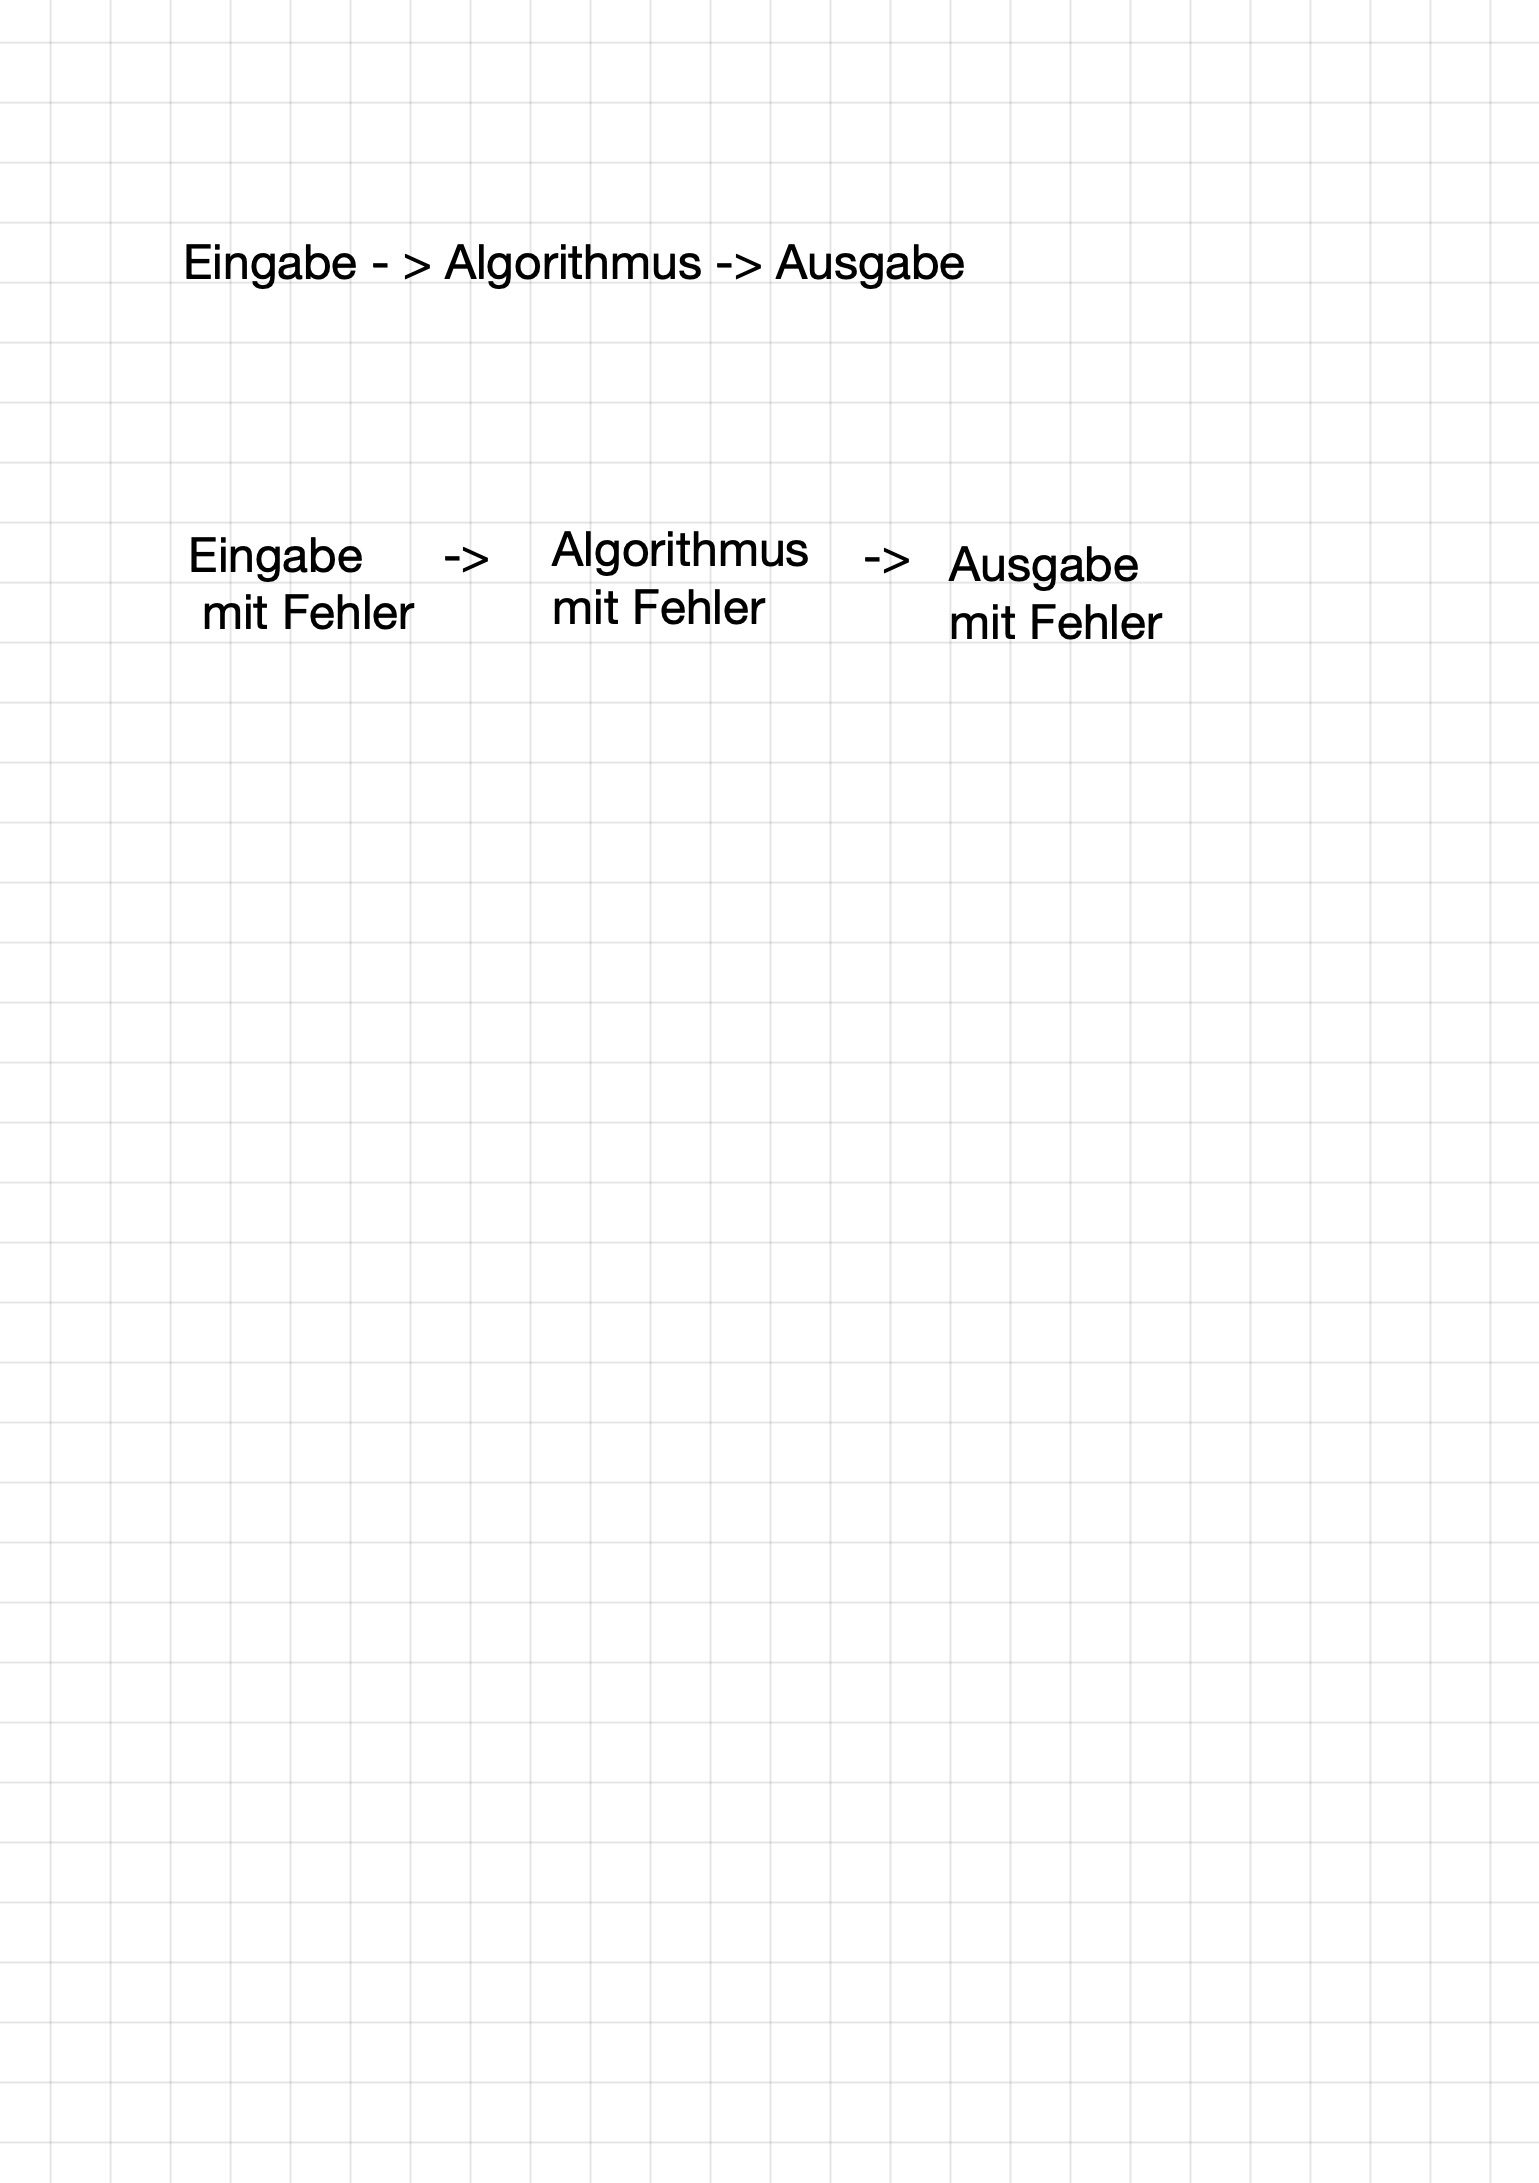
\includegraphics[width=0.7\textwidth]{images/fehler}\end{figure}
 \end{frame}

\begin{frame}
    \frametitle{Angewandte Mathematik}
\framesubtitle{Fehleranalyse}
    \begin{block}{Konditionszahl}
 Die Kondition beschreibt  die Abhängigkeit der Lösung eines Problems von der Störung der Eingangsdaten.  Die Konditionszahl stellt ein Maß für diese Abhängigkeit dar. Sie beschreibt das Verhältnis von  $E:= \{\widetilde{x} \; | \; ||\widetilde{x} -x || \leq eps ||x|| \}$ zu $R: = \{f(\widetilde{x}) \; | \; \widetilde{x} \in E \}$.
\end{block}
\begin{figure}[H]
      \centering
    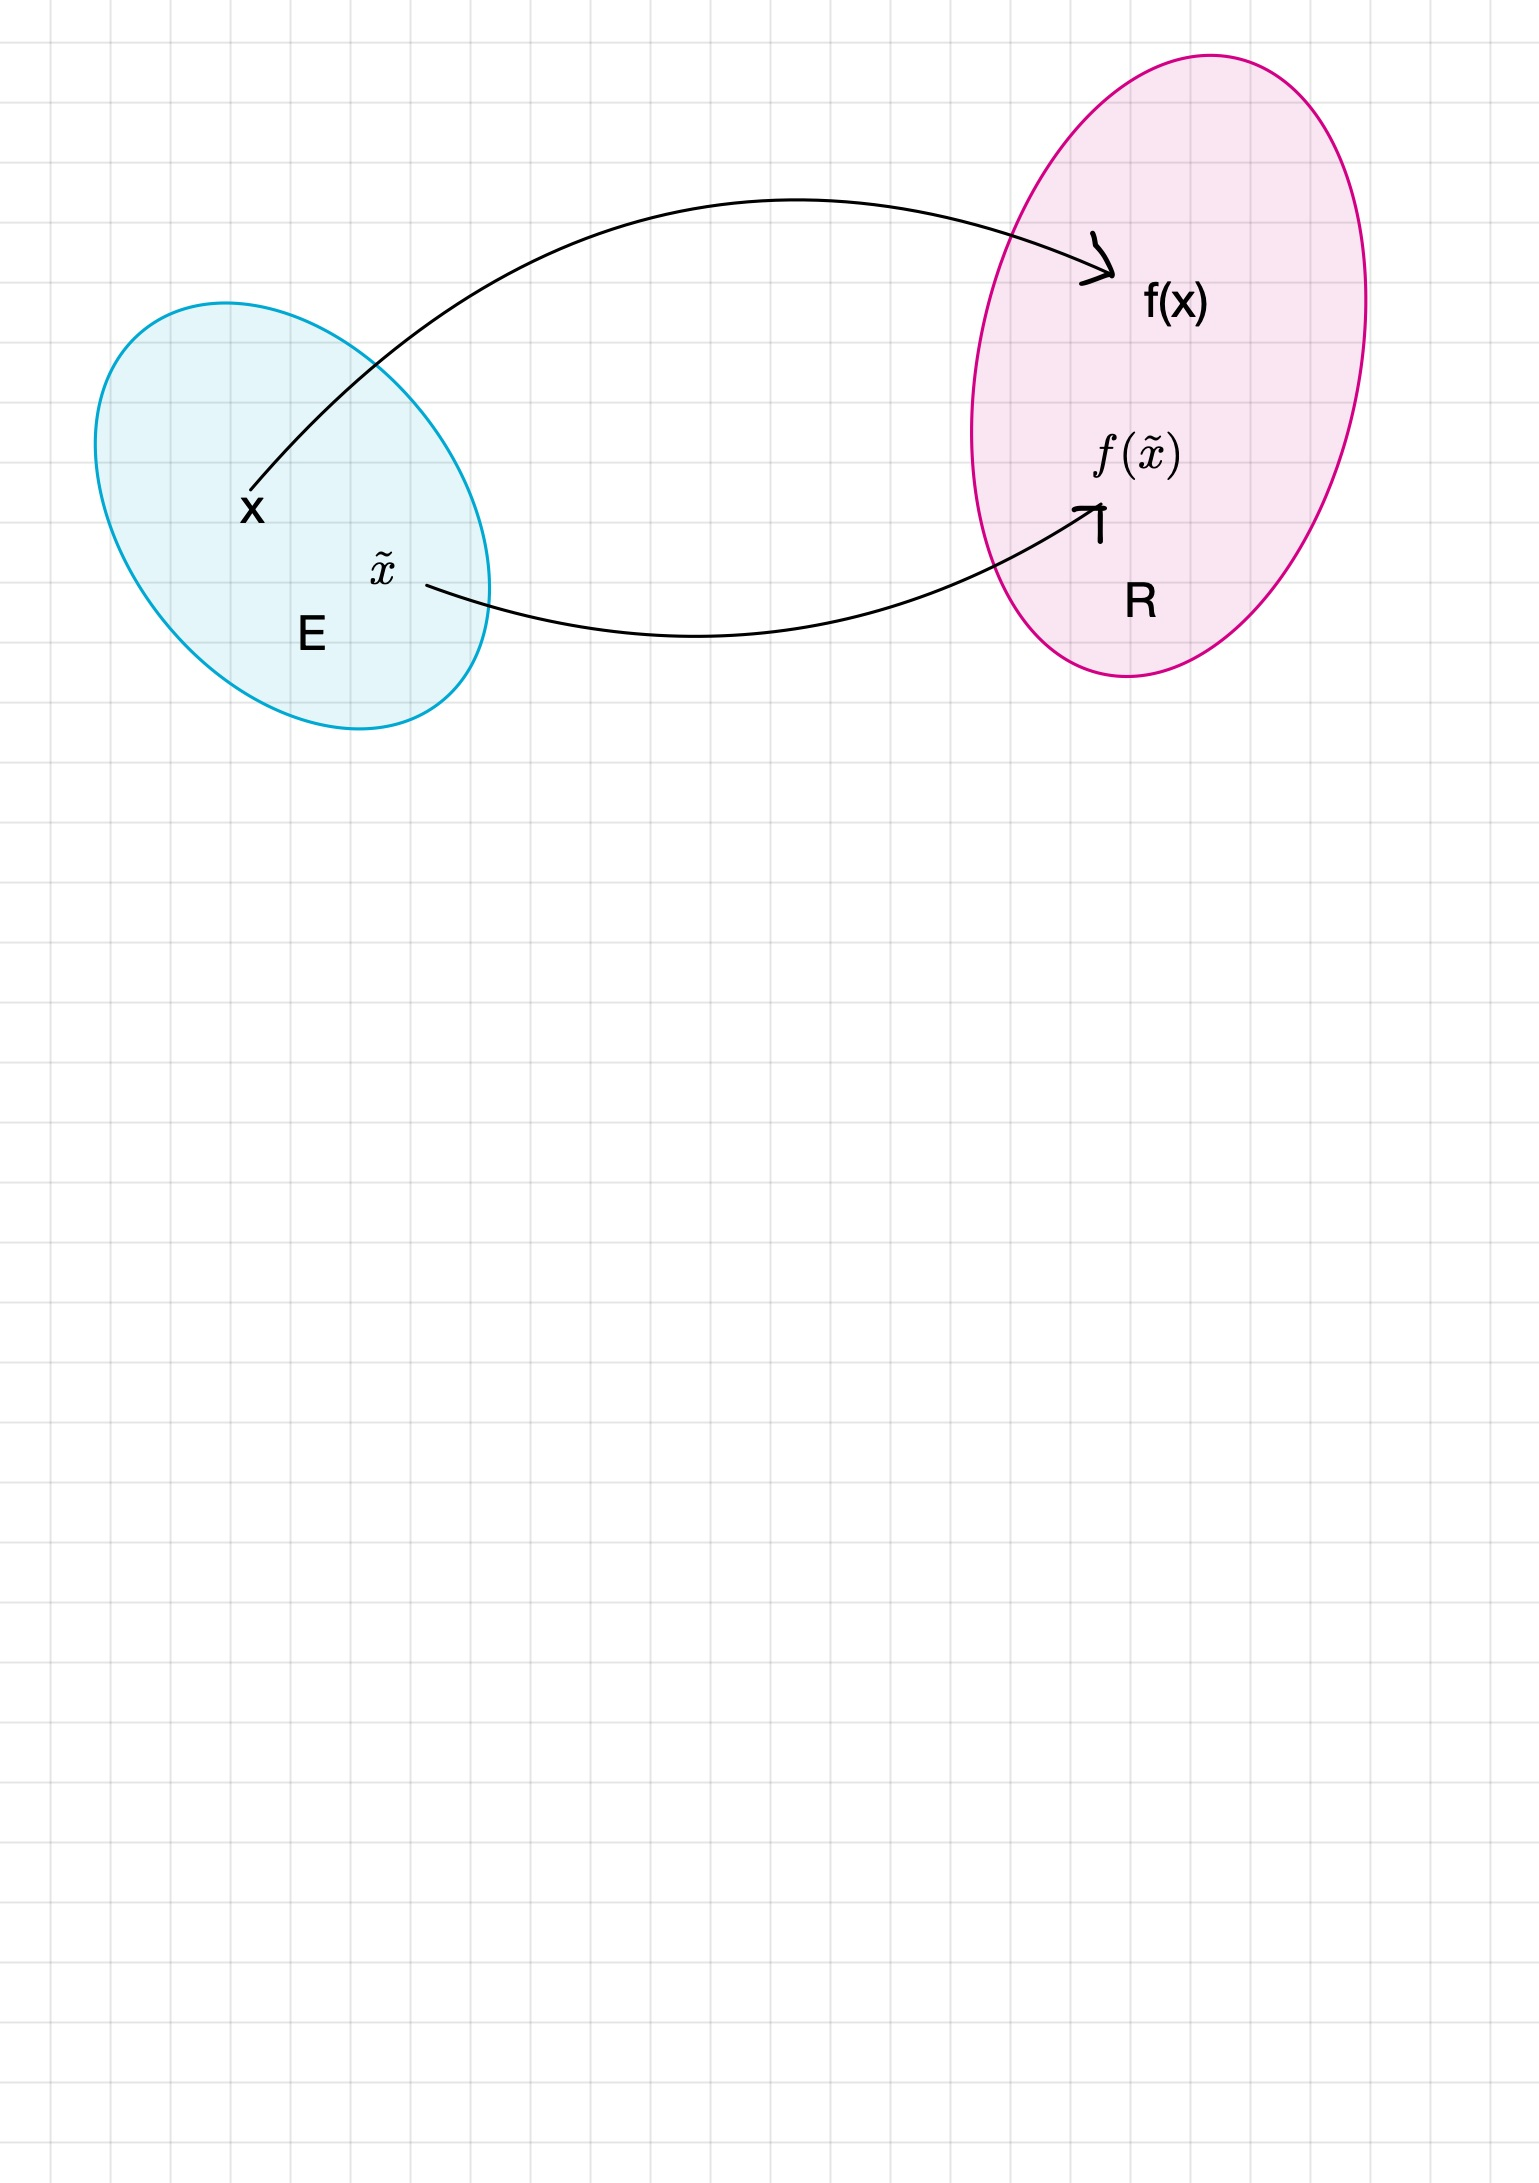
\includegraphics[width=0.8\textwidth]{images/kondition}
      \caption{}
\end{figure}

 \end{frame}



\begin{frame}
    \frametitle{Angewandte Mathematik}
\framesubtitle{Fehleranalyse}
    \begin{block}{Kondition eines Problems}
Die absolute Konditionierung eines Problems $(f,x)$ ist die Kleinste Zahl $\kappa_{abs}$ mit 
\begin{align*}
|| f(x) - f(\widetilde{x}) || \leq \kappa_{abs} || x - \widetilde{x} || , \;  \widetilde{x} \to x
\end{align*}
\end{block}

    \begin{block}{Kondition eines Problems}
Die relative  Konditionierung eines Problems $(f,x)$ ist die Kleinste Zahl $\kappa_{rel}$ mit 
\begin{align*}
\frac{|| f(x) - f(\widetilde{x}) ||}{||f(x) || } \leq \kappa_{rel} \frac{|| x - \widetilde{x} ||}{||x||} , \; \widetilde{x} \to x
\end{align*}
\end{block}

 \end{frame}





%\begin{frame}
%    \frametitle{Angewandte Mathematik}
%\framesubtitle{Fehleranalyse}
%    \begin{block}{Stabilität}
%Für eine Gleikommarealisierung $\hat{f}$ eines Algorithmus zur Lösung des Problems $(f,x)$ mit relativer Konditionszahl $\kappa_rel$ ist der Stabilitätsindikator definiert als die kleinste Zahl $\sigma \geq 0$ mit 
%\begin{align*}
%\frac{|| \hat{f}(\widetilde{x}) - f(\widetilde{x}) ||}{||f(\widetilde{x}) || } \leq \sigma  \kappa_{rel} eps , \; eps \to 0
%\end{align*}
%für alle $\widetilde{x} \in E$
%\end{block}
%    \begin{block}{Stabilität eines Algorithmus}
%Der Algorithmus $\hat{f}$ heisst stabil, wenn $\sigma$ kleiner ist als die Anzahl der hintereinander ausgeführten Elementaroperationen. 
%\end{block}
% \end{frame}



 \begin{frame}
    \frametitle{Angewandte Mathematik}
\framesubtitle{Mittelwertsatz}
    \begin{block}{Mittelwertsatz}
Ist $f: U \to \mathbb{R}$ eine differenziertere Funktion und $a,b \in U$ Punkte, deren Verbindungsstrecke in $U$ verläuft. Dann gibt gibt es einen Punkt $\xi$ auf dieser Verbindungsstrecke mit
\begin{align*}
f(b) - f(a) = df(\xi)(b-a) = f'(\xi) (b-a)
\end{align*}
\end{block}
 \end{frame}



\begin{frame}
    \frametitle{Angewandte Mathematik}
\framesubtitle{Mittelwertsatz}
    \begin{block}{Beweis Mittelwertsatz}
Die Verbindungsstrecke ist gegeben durch $\gamma(t) := a + t(b-a)$ mit $t \in [0,1]$. 
Für $F:= f \circ \gamma : [0,1] \to \mathbb{R}$ gilt $f(b) - f(a)= F(1) - F(0)$.
Nach der Kettenregel ist $F$ differenzierbar. Mit dem eindimensionalen Mittelwertsatz gibt es also ein $\tau \in (0,1)$ mit
$F(1) - F(0) = F'(\tau)$. Mit der Kettenregel folgt $F'(\tau) = df(\gamma(\tau)) (b-a)$ und somit folgt mit $\xi= \gamma(\tau)$ die Behauptung.
\end{block}



\begin{figure}[H]
    \centering
  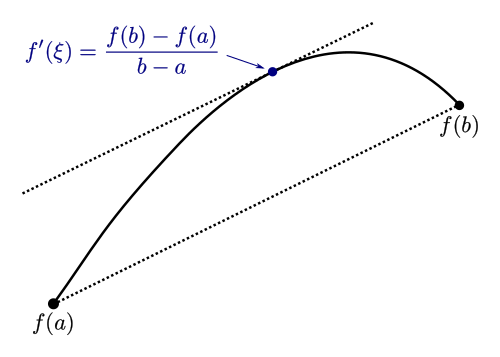
\includegraphics[width=0.5\textwidth]{images/Mittelwertsatz3.png}
\end{figure}

 \end{frame}



 \begin{frame}
    \frametitle{Angewandte Mathematik}
\framesubtitle{Backpropagation}
    \begin{block}{Konditionszahl}
Ist $f : U \to \mathbb{R}^m$ differnzierbar, so lässt dich mit dem Mittelwertsatz die Konditionszahlen berechnen durch
\begin{align*}
& \kappa = || f'(x) || \\
& \kappa_{rel} = \frac{||x||}{|| f(x)||} ||f'(x) ||
\end{align*}
mit der Operatornorm 
$||h|| : = \sup_{||x|| =  1} ||h(x)||$

\end{block}
 \end{frame}

\begin{frame}
    \frametitle{Angewandte Mathematik}
\framesubtitle{Backpropagation}
    \begin{block}{Konditionszahl Addition/Subtraction}
Für $f:(x,y):= x \pm y$ ist $f'(x,y) = (1,\pm 1)$ und dem Betrag als Norm auf $\mathbb{R}$  und der Norm $||(x,y)|| := |x| + |y|$ ist 
\begin{align*}
& \kappa = 2 \\
& \kappa_{rel} = 2\frac{|a| + |b| }{|a \pm b|}
\end{align*}
Für die Addition ist  $\kappa_{rel} = 2$ und damit gut konditioniert.
Für die Subtraktion zweier fast gleich großer Zahlen ist $|a - b| << |a| + |b|$ und damit ist in diesem Fall $\kappa_{rel} >> 1$ und damit schlecht konditioniert. 
\end{block}
 \end{frame}




 \begin{frame}
    \frametitle{Angewandte Mathematik}
    \framesubtitle{Numerische Software}
    \begin{block}{Message Passing Interface (MPI)}
          MPI ist ein Standard für die Kommunikation zwischen Prozessen in einem parallelen Rechensystem.
          Es ermöglicht die Entwicklung von standardtisierten parallelen Anwendungen, die auf verschiedenen Rechnerarchitekturen laufen können.
    \end{block}
\end{frame}



\begin{frame}
    \frametitle{Angewandte Mathematik}
    \framesubtitle{Numerische Software}
    \begin{block}{Message Passing Interface (MPI)}
            \begin{itemize}
                \item \textbf{Punkt-zu-Punkt-Kommunikation:} Direkte Kommunikation zwischen zwei Prozessen mittels Senden und Empfangen von Nachrichten.
                \item \textbf{Kollektive Kommunikation:} Kommunikation zwischen einer Gruppe von Prozessen, z.B. Broadcast, Scatter, Gather und Reduce.
                \item \textbf{Synchronisation:} Mechanismen zur Synchronisation von Prozessen, z.B. Barrieren.
                \item \textbf{Kommunikatoren:} Gruppen von Prozessen, die miteinander kommunizieren können.
                \item \textbf{Rang:} Jeder Prozess in einem Kommunikator hat einen eindeutigen Rang, der zur Identifikation dient.
            \end{itemize}
    \end{block}
\end{frame}

\begin{frame}
    \frametitle{Angewandte Mathematik}
    \framesubtitle{Numerische Software}
    \begin{block}{Portable, Extensible Toolkit for Scientific Computation (PETSc)}
            PETSc ist eine Bibliothek für die Lösung wissenschaftlicher Rechenprobleme, die auf parallelen und verteilten Systemen ausgeführt werden.
            Bietet Werkzeuge für die Entwicklung von skalierbaren und effizienten numerischen Anwendungen.
            
            \begin{itemize}
                \item PETSc nutzt MPI für die Kommunikation zwischen Prozessen in parallelen Umgebungen.
                \item Unterstützt Punkt-zu-Punkt- und kollektive Kommunikation, um Daten zwischen Prozessen auszutauschen.
                \item Ermöglicht die Verteilung von Matrizen und Vektoren über mehrere Prozesse.
                \item Lineare und nichtlineare Gleichungslöser
                \item Eigenwertproblemlöser
                \item Zeitabhängige Probleme
                \item Preconditioner für die Beschleunigung der Konvergenz
            \end{itemize}
    \end{block}
\end{frame}



\begin{frame}
    \frametitle{Angewandte Mathematik}
    \framesubtitle{Numerische Software}
    \begin{block}{NumPy}
            NumPy ist eine Bibliothek für die Programmiersprache Python, die Unterstützung für große, mehrdimensionale Arrays und Matrizen bietet.
            Ermöglicht effiziente numerische Berechnungen und Datenmanipulationen.
    \end{block}
\end{frame}

\begin{frame}
    \frametitle{Angewandte Mathematik}
    \framesubtitle{Numerische Software}
    \begin{block}{Grundprinzipien von NumPy}
        \begin{itemize}
            \item \textbf{Arrays:} NumPy bietet das `ndarray`-Objekt, das effiziente Speicher- und Rechenoperationen ermöglicht.
            \item \textbf{Broadcasting:} Ermöglicht die Durchführung von Operationen auf Arrays unterschiedlicher Größe.
            \item \textbf{Vektorisierung:} Vermeidet explizite Schleifen durch die Anwendung von Operationen auf ganze Arrays.
            \item \textbf{Universelle Funktionen (ufuncs):} Funktionen, die elementweise Operationen auf Arrays durchführen.
        \end{itemize}
    \end{block}
\end{frame}

\begin{frame}
    \frametitle{Angewandte Mathematik}
    \framesubtitle{Numerische Software}
    \begin{block}{Vorteile und Anwendungsgebiete von NumPy}
            \begin{itemize}
                \item Hohe Leistung durch Implementierung in C
                \item Umfangreiche Bibliothek von mathematischen Funktionen
                \item Integration mit anderen wissenschaftlichen Python-Bibliotheken wie SciPy und Matplotlib
        \end{itemize}
    \end{block}
\end{frame}

\end{document}

